% -*- root: ../thesis.tex -*-
%!TEX root = ../thesis.tex
% ******************************* Thesis Chapter 7 ****************************

% ----------------------- paths to graphics ------------------------

% change according to folder and file names
\graphicspath{{8/figures/}}
% ----------------------- contents from here ------------------------


\section{Further generalizations}
The works presented in this thesis only scratched the surface of how mixtures can be helpful and how to identify them.
We are still exploring ways to identify larger classes of functions which can be evaluated as scale-mixture.
In particular, the simple connection with the \acf{MGF} of a distribution is a promising way as it allow working not only with continuous but discrete variables (as presented in Chapter \ref{ch:multiclass}).

Another promising way is to identify when some augmented variables can be marginalized out while keeping the conditional conjugacy of the model.
An example of this is quickly given in the section~\ref{sec:improvemulticlass}.

\section{Double bounds for intricate latent GPs}

The model developed in Chapter~\ref{ch:multiclass} paves the ways to work with multi-latent models and hierarchical augmentations.
Another model explored is the heteroscedastic Gaussian regression model which was already explored in \cite{wangGaussianProcessRegression2012}.
By having two latent \ac{GPs} $f$ and $g$, one can model simultaneously the mean and the variance.
An important choice is the link between $g$ and the likelihood variance $\epsilon^2$.
The most popular link is the exponential link, i.e. $\epsilon^2(x) = \exp(g(x))$, however to be able to apply our augmentations, we use the link $\epsilon^2(x) = \left(\lambda \sigma(g(x))\right)^{-1}$.
The likelihood becomes :
\begin{align}
    p(y|f,g,\lambda) = \frac{\sqrt{\lambda \sigma(g)}}{\sqrt{2\pi}}\exp\left(-\frac{\lambda \sigma(g)(y-f)^2}{2}\right).\label{eq:hetero_lik}
\end{align}

The augmentations are straightforward and quite similar to the multi-class ones from Chapter~\ref{ch:multiclass}.
\begin{align*}
    \exp\left(-\frac{\lambda\sigma(g)(y-f)^2}{2}\right) =& \exp\left(\frac{\lambda(\sigma(-g) -1)(y-f^2)}{2}\right)\\
    =&\sum_{n=0}^\infty \sigma^n(-g)\Po \left(n~\middle|~\frac{\lambda(y-f)^2}{2}\right),
\end{align*}
where we used the \ac{MGF} of the Poisson distribution.
Now using the P\'olya-Gamma augmentation we get the final augmented likelihood:
\begin{align*}
    p(y,n,\omega\mid f,g,\lambda) = \frac{\sqrt{\lambda}}{2^n\sqrt{\pi}}\exp\left(\frac{1}{2}\left(g\left(\frac{1}{2}-n\right) - \frac{g^2}{\omega}\right)\right)\PG \left(\omega \mid \half + n, 0\right) \Po \left(n \mid \lambda\frac{(y-f)^2}{2}\right)
\end{align*}
The interesting part about this augmented likelihood is that although it is conditionally conjugate in $g$, $\omega$ and $n$, it is not clear how it works for $f$.
It turns out that the Gibbs sampler for this model is actually extremely simple as for the full-conditional of $f$ we can simply marginalize $n$ and $\omega$, return to the original likelihood, which is conditionally conjugate, and perform a \textbf{collapsed} step for the Gibbs sampler.

However, as underlined in Section~\ref{sec:cavi}, the \ac{CAVI} updates need the full-conditionals of the model, and it is not clear how a marginalized version can work.
To solve the problem we define an additional bound on the original \ac{ELBO}:
\begin{align*}
    \KL{q(\boldf)q(\boldg)}{p(\boldf,\boldg|\boldy)}\leq& \min_{q(\boldg)}-\expec{q(\boldg)}{\expec{q(\boldf)}{\log p(\boldy|\boldf,\boldg)}} + \KL{q(\boldf)q(\boldg)}{p(\boldf)p(\boldg)}\\
    =& \min_{q(\boldg)}-\expec{q(\boldg)}{\log p(\boldy|\boldg, \bmu^*_f,\bSigma^*_f)} + \KL{q(\boldg)}{p(\boldg)} + \operatorname{KL}_f^* = \mathcal{F}_1.
\end{align*}
$p(\boldy|\boldg, \bmu^*_f, \bSigma^*_f)$ and $\mathrm{KL}^*_f$ are expectations computed with the optimal $q^*(\boldf)$.
We can now use the augmentation on the expected log-likelihood (in practice we simply modified $(y_i-f_i)^2$ by $(y_i - \mu_i^2)^2 + \Sigma_{ii}$).

\begin{align*}
    \mathcal{F}_1 \leq \min_{q(\boldg)q(\bomega,\bn)} \expec{q(\boldg)q(\bomega,\bn)}{\log p(\bomega,\bn,\boldy|\boldg,\bmu_f^*,\bSigma_f^*)} + \KL{q(\boldg)}{p(\boldg)} + \operatorname{KL}_f^*=\mathcal{F}_2
\end{align*}

It is straightforward to find the optimal variational distributions $q^*(\boldg)$ and $q^*(\bomega,\bn)$ minimizing $\mathcal{F}_2$ which allows us to use \ac{CAVI} updates.
Then, injecting the optimal distributions we can derive the optimal $\bmu_f^*$ and $\bSigma_f^*$, which once again, are obtainable in closed-form.


\section{Using Hamilton Monte Carlo on the augmented model}

The Gibbs sampler in the experiments of Chapters~\ref{ch:classification} and \ref{ch:general} outperform the state-of-the-art \ac{HMC} algorithm introduced in Section~\ref{sec:hmc}.
A natural question to ask is: is the performance gain due to the augmentation or to the use of a Gibbs sampler?
A first answer to this is that the \ac{HMC} sampler is not well adapted to the augmentation due to the large increase of dimensionality of the model.
For $N$ observations, it is at least $N$ more dimensions to add, making gradients computations and the algorithm parameters tuning more complicated and expensive.
The second issue with \ac{HMC} with the augmented model is that the \ac{pdf} of the augmented variables is not always available in closed-form.
For example, to estimate the probability of a P\'olya-Gamma variables, a truncated series is used.
This is not only limited in accuracy but also much more expensive to compute.
But if one perseveres, the Figure~\ref{fig:hmc_vs_gibbs} shows the auto-correlation plots on a toy \ac{GP} classification problem.

\begin{figure}
    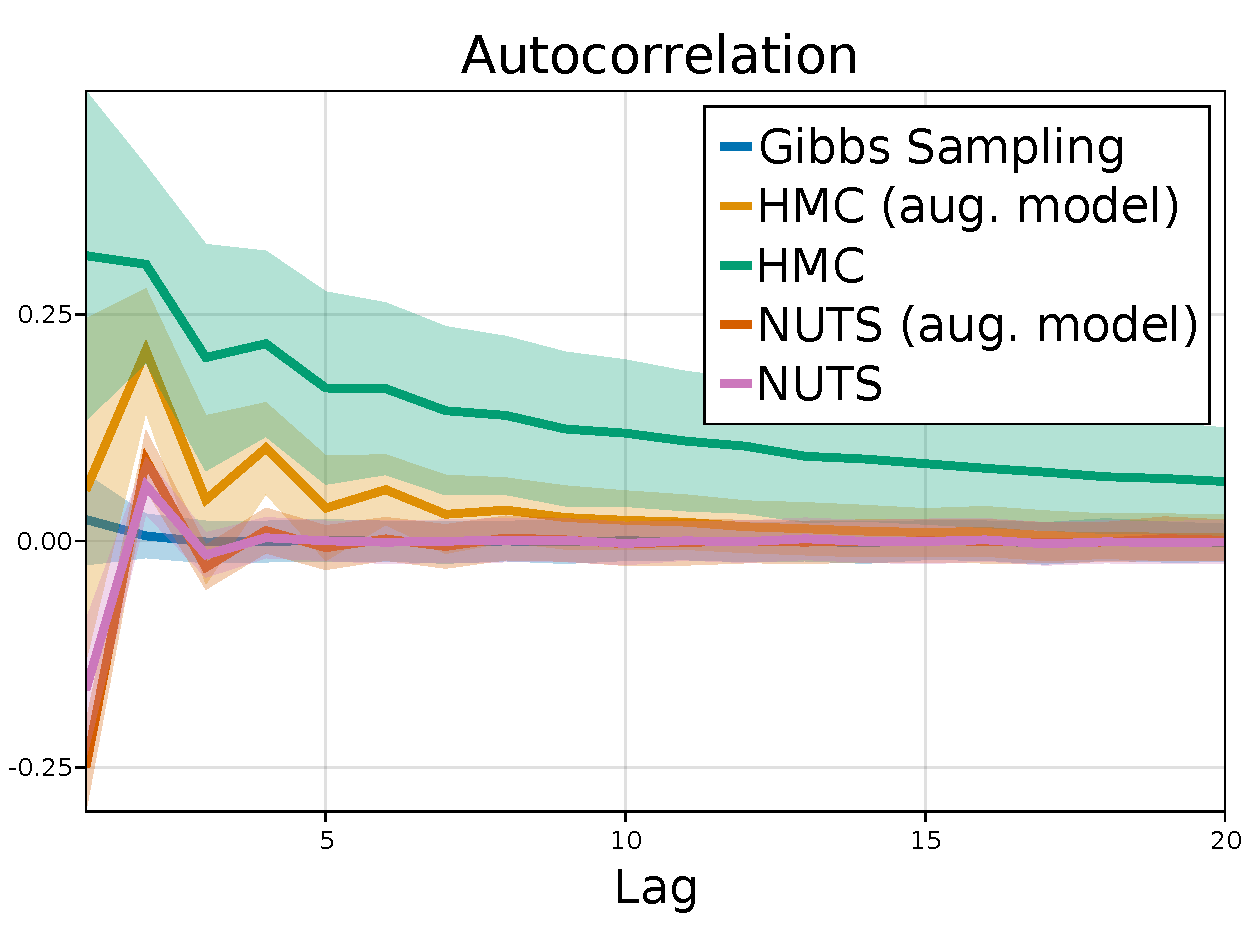
\includegraphics[width=\textwidth]{./chapters/8_discussions/figures/autocorrelation.pdf}
    \caption{Auto-correlation of a Gibbs sampler and \ac{NUTS} on the augmented model, and of \ac{NUTS} on the original model}
    \label{fig:hmc_vs_gibbs}
\end{figure}


\section{Improvements on the Multi-Class Classification}
\label{sec:improvemulticlass}
We recently figured that there were additional ways to improve the augmented models and the associated inference.

\subsection{Simplex for the multi-class classification}
\label{sec:simplex}
In Chapter \ref{ch:multiclass}, one of the possible concerns regarding the model is that $\lambda$ has the improper prior $1_{0,\infty}$, which is a proper measure but is not normalizable.
It should be noted that since the resulting posterior is valid, no problem should arise, but from a purely Bayesian perspective this can be dissatisfactory.
This improper prior rises from the fact that the model we are using is ill-conditioned.
Given $K$ classes, only $K-1$ latent \ac{GP} are needed since we have the additional constraint that $\sum_{k=1}^K p(y=k|\boldf) = 1$.
Using this formulation we get the following likelihood:
\begin{align}
    p(y=k|\{f_k\}_{k=1}^{K-1}) = \left\{
        \begin{array}{cc}
            \frac{\sigma(f_k)}{D + \sum_{i=1}^{K-1}\sigma(f_i)}, & \mathrm{if}\; 1 \leq k < K - 1\\
            \frac{D}{D + \sum_{i=1}^{K-1}\sigma(f_i)}, & \mathrm{if}\; k = K - 1 \\
    \end{array}
    \right.,
\end{align}
where $D \in [0, 1]$.

Using this formulation, the first augmentation that led to an improper prior :
\begin{align*}
    \frac{1}{ \sum_{i=1}^{K} \sigma(f_i)} = \int_0^\infty e^{-\lambda  \sum_{i=1}^{K} \sigma(f_i)}d\lambda
\end{align*}
becomes the known \ac{MGF} of a Gamma distribution with a proper mixture:
\begin{align*}
    \frac{1}{D + \sum_{i=1}^{K-1} \sigma(f_i)} =& \frac{1}{D + K - 1 - \sum_{i=1}^{K-1} \sigma(-f_i)}\\
    =& \frac{1}{D + K - 1}\int_0^\infty e^{-\lambda \sum_{i=1}^{K-1} \sigma(-f_i)}\Ga \left(1, \frac{1}{D + K - 1}\right)d\lambda
\end{align*}
Note that an important condition to use the \ac{MGF} is that $\sum_{i=1}^{K-1} \sigma(-f_i) < D + K - 1$ which is true as long as $D > 0$.
This condition would not necessarily hold if we used the over-parametrized version which would lead to $\sum_{i=1}^{K} \sigma(-f_i) < K$ (not true when taking the limits $\forall i,\;f_i \rightarrow -\infty$).

From there the derivations are the same, i.e. using the \ac{MGF} of a Poisson distribution and finally using the P\'olya-Gamma augmentation.
Unfortunately we did not run any experiments to explore if one parametrization was more accurate or efficient than another.

\subsection{Marginalizing out variables}
In the augmentation derived in Chapter~\ref{ch:multiclass}, we add $2K + 1$ new variables per observation: $\lambda$, $\{n_i\}_{i=1}^K$ and $\{\omega_i\}_{i=1}^K$.
However, we can reduce this number to $2K$ by marginalizing out one of the variables and therefore avoiding complicated inner loops.
When deriving the augmentations, at some point, one ends up with the following augmented likelihood:
\begin{align}
    p(y=k|\{f_i\}_{i=1}^K) = \sigma(f_k) \prod_{i=1}^K \sigma(-f_i)^{n_i} \Po (n_i|\lambda).
\end{align}
We can marginalize out the $\lambda$:
\begin{align}
    \int_{0}^\infty \prod_{i=1}^K \sigma(-f_i)^{n_i} \Po (n_i|\lambda)d\lambda =& \frac{1}{\prod_{i=1}^K n_i!}\int_{0}^\infty \lambda^{\sum_{i=1}^K n_i}e^{-K\lambda}d\lambda \nonumber\\
    =& \frac{K^{-\sum_{i=1}^K n_i}}{\prod_{i=1}^K n_i!}\prod_{i=1}^K \sigma(-f_i)^{n_i} \int_{0}^\infty (K\lambda)^{\sum_{i=1}^K \sigma(f_i)}e^{-K\lambda}d\lambda \nonumber\\
    =& \Gamma(1 + \sum_{i=1}^K n_i) \prod_{i=1}^K \left(\frac{\sigma(-f_i)}{K}\right)^{n_i}\frac{1}{n_i!} \label{eq:NM}
\end{align}

Which is proportional to a negative multinomial $\operatorname{NM}(x_0, \boldsymbol{p})$ with parameters $x_0=1$, $\boldsymbol{p}=\left\{\frac{\sigma(-f_i)}{K}\right\}_{i=1}^K$:
\begin{align*}
    \operatorname{NM}(\bx|x_0,\boldsymbol{p}) = \Gamma\left(\sum_{i=0}^K x_i\right) \frac{p_0^{x_0}}{\Gamma(x_0)}\prod_{i=1}^K \frac{p_i^{x_i}}{x_i!}   
\end{align*}
where $p_0 = 1 - \sum_{i=1}^K p_i$.
Note that $p_0$ is the missing normalization constant in Equation~\ref{eq:NM} and that it would directly depend on $\{f_i\}_{i=1}^K$, making the likelihood non-normalizable.
The effect mentioned in Section~\ref{sec:simplex} is still propagated to the marginalized augmented likelihood.

More interestingly, all these derivations could have been avoided by noticing that the \ac{MGF} of a negative binomial distribution is given by:
\begin{align*}
    \operatorname{MGF}_{\operatorname{NM}(x_0,\boldsymbol{p})}(\boldsymbol{t}) = \left(\frac{p_0}{1-\sum_{i=1}^K p_k e^{t_i}}\right)^{x_0},
\end{align*}
This makes it even easier to derive the correctly parametrized model proposed in Section~\ref{sec:simplex}.
Quickly identifying the terms in the \ac{MGF}, the augmented likelihood would be:
\begin{align*}
    p\left(y=k,\{n_i\}_{i=1}^{K-1}|\{f_i\}_{i=1}^{K-1}\right) = \frac{\sigma(f_k)}{D}\left(\prod_{i=1}^{K-1}\sigma(-f_i)^{n_i}\right)\operatorname{NM}\left(\boldsymbol{n}\mid 1, \left\{\frac{1}{D+K-1}\right\}_{i=1}^{K-1}\right),
\end{align*}
where we set $\sigma(f_K) = D$.

\subsection{Reformulating the logistic-softmax link}

Another issue that rose from this paper was the logistic-softmax link limitations, especially in the many-class problem.
Because of the bounds of the logistic function, extremely high value of $f_i$ are needed to reach class prediction probability of $1$.
This could be easily solved by using a scaled logistic function instead.
One could add $K$ hyperparameters $\btheta$ such that the likelihood is written as:
\begin{align*}
    p(y=k|\{f_i\}_{i=1}^K,\btheta) = \frac{\theta_k \sigma(f_k)}{\sum_{i=1}^K \theta_i \sigma(f_i)}.
\end{align*}
The $\btheta$ parameters can be optimized using the \ac{ELBO} as the other hyperparameters.
These can also provide some information about each class, a high $\theta_i$ means that the $i$-th class has zones of very high confidence.

% ---------------------------------------------------------------------------
% ----------------------- end of thesis sub-document ------------------------
% ---------------------------------------------------------------------------
